%%%%%%%%%%%%%%%%%%%%%%%%%%%%%%%%%%%%%%%%%
% Dreuw & Deselaer's Poster
% LaTeX Template
% Version 1.0 (11/04/13)
%
% Created by:
% Philippe Dreuw and Thomas Deselaers
% http://www-i6.informatik.rwth-aachen.de/~dreuw/latexbeamerposter.php
%
% This template has been downloaded from:
% http://www.LaTeXTemplates.com
%
% License:
% CC BY-NC-SA 3.0 (http://creativecommons.org/licenses/by-nc-sa/3.0/)
%
%%%%%%%%%%%%%%%%%%%%%%%%%%%%%%%%%%%%%%%%%

%----------------------------------------------------------------------------------------
%	PACKAGES AND OTHER DOCUMENT CONFIGURATIONS
%----------------------------------------------------------------------------------------

\documentclass[final,hyperref={pdfpagelabels=false}]{beamer}

\usepackage[orientation=portrait,size=a0,scale=1.4,debug]{beamerposter} % Use the beamerposter package for laying out the poster with a portrait orientation and an a0 paper size

\usetheme{I6pd2} % Use the I6pd2 theme supplied with this template

\usepackage[english]{babel} % English language/hyphenation

\usepackage{amsmath,amsthm,amssymb,latexsym} % For including math equations, theorems, symbols, etc

%\usepackage{times}\usefonttheme{professionalfonts}  % Uncomment to use Times as the main font
%\usefonttheme[onlymath]{serif} % Uncomment to use a Serif font within math environments

\boldmath % Use bold for everything within the math environment

\usepackage{booktabs} % Top and bottom rules for tables
\usepackage{subfigure} 

\graphicspath{{figures/}} % Location of the graphics files

\usecaptiontemplate{\small\structure{\insertcaptionname~\insertcaptionnumber: }\insertcaption} % A fix for figure numbering

%----------------------------------------------------------------------------------------
%	TITLE SECTION 
%----------------------------------------------------------------------------------------

\title{\huge (2-F-56) Histogram of Gradient Orientations of Signal Plots applied to Brain Computer Interfaces}
\author{Ramele Rodrigo, Santos Juan Miguel, Villar Ana Julia}
\institute[Instituto Tecnológico de Buenos Aires]{Computer Engineering Department,Graduate School of Engineering, Buenos Aires, Argentina}
\date[May. 22nd, 2018]{May. 22nd, 2018}

%----------------------------------------------------------------------------------------
%	FOOTER TEXT
%----------------------------------------------------------------------------------------
\newcommand{\leftfoot}{https://www.itba.edu.ar/id/centro-de-inteligencia-computacional/} % Left footer text

\newcommand{\rightfoot}{rramele@itba.edu.ar} % Right footer text
\newlength{\columnheight}
\setlength{\columnheight}{115cm}
%----------------------------------------------------------------------------------------

\begin{document}

\addtobeamertemplate{block end}{}{\vspace*{2ex}} % White space under blocks

\begin{frame}[t] % The whole poster is enclosed in one beamer frame

\begin{columns}[t] % The whole poster consists of two major columns, each of which can be subdivided further with another \begin{columns} block - the [t] argument aligns each column's content to the top

\begin{column}{.02\textwidth}\end{column} % Empty spacer column

\begin{column}{.465\textwidth} % The first column

%%----------------------------------------------------------------------------------------
%%	OBJECTIVES
%%----------------------------------------------------------------------------------------
%
%\begin{block}{Objectives}
%
%\begin{enumerate}
%\item Donec fringilla, velit id lobortis commodo, eros dui consectetur mi, ut interdum lorem dui sed mauris.
%\item Nulla ac nulla rhoncus est bibendum ullamcorper:
%\item Quisque vestibulum, nisl sit amet gravida ultricies dis parturient montes, nascetur ridiculus musobortis commodo, eros dui consectetur mi.
%\end{enumerate}
%
%\end{block}

%----------------------------------------------------------------------------------------
%	INTRODUCTION
%----------------------------------------------------------------------------------------
            
\begin{block}{Introduction}

\begin{itemize}
\item \textbf{Where are the Waveforms?}
\begin{itemize}
\item Around $71.2\%$ of BCI Research is based on Noninvasive EEG \textsuperscript{[1]}
\end{itemize}
\item EEG has traditionally focused on temporal waveforms. Few methods exploited automatically signal waveforms:
\begin{itemize}
\item Matching Pursuit (Mallat 1993)
\item Permutation Entropy (Bandt-Pompe 2002)
\item Slope Horizontal Chain Code\textsuperscript{[2]}.
\item Merging of Increasing and Descending Sequences\textsuperscript{[3]}.
\end{itemize}
\item Clinical atlases and guidelines were developed based on waveforms.   
\begin{itemize}
\item More interaction between BCI stakeholders should be fostered\textsuperscript{[7]}.
\end{itemize}
\end{itemize}

\end{block}

%----------------------------------------------------------------------------------------
%	MATERIALS
%----------------------------------------------------------------------------------------

\begin{block}{Materials}

\begin{columns} % Subdivide the first main column
\begin{column}{.54\textwidth} % The first subdivided column within the first main column
\begin{itemize}
\item Research Oriented Digital EEG Device
\begin{itemize}
\item g.Nautilus, 8-channel, wet electrodes, g.Tec.
\end{itemize}
\item Open Source Platform and Software
\begin{itemize}
\item OpenVibe
\item Matlab
\item C++ VLFeat Computer Vision Library.
\end{itemize}

\end{itemize}
\end{column}

\begin{column}{.43\textwidth} % The second subdivided column within the first main column
\centering
\begin{figure}
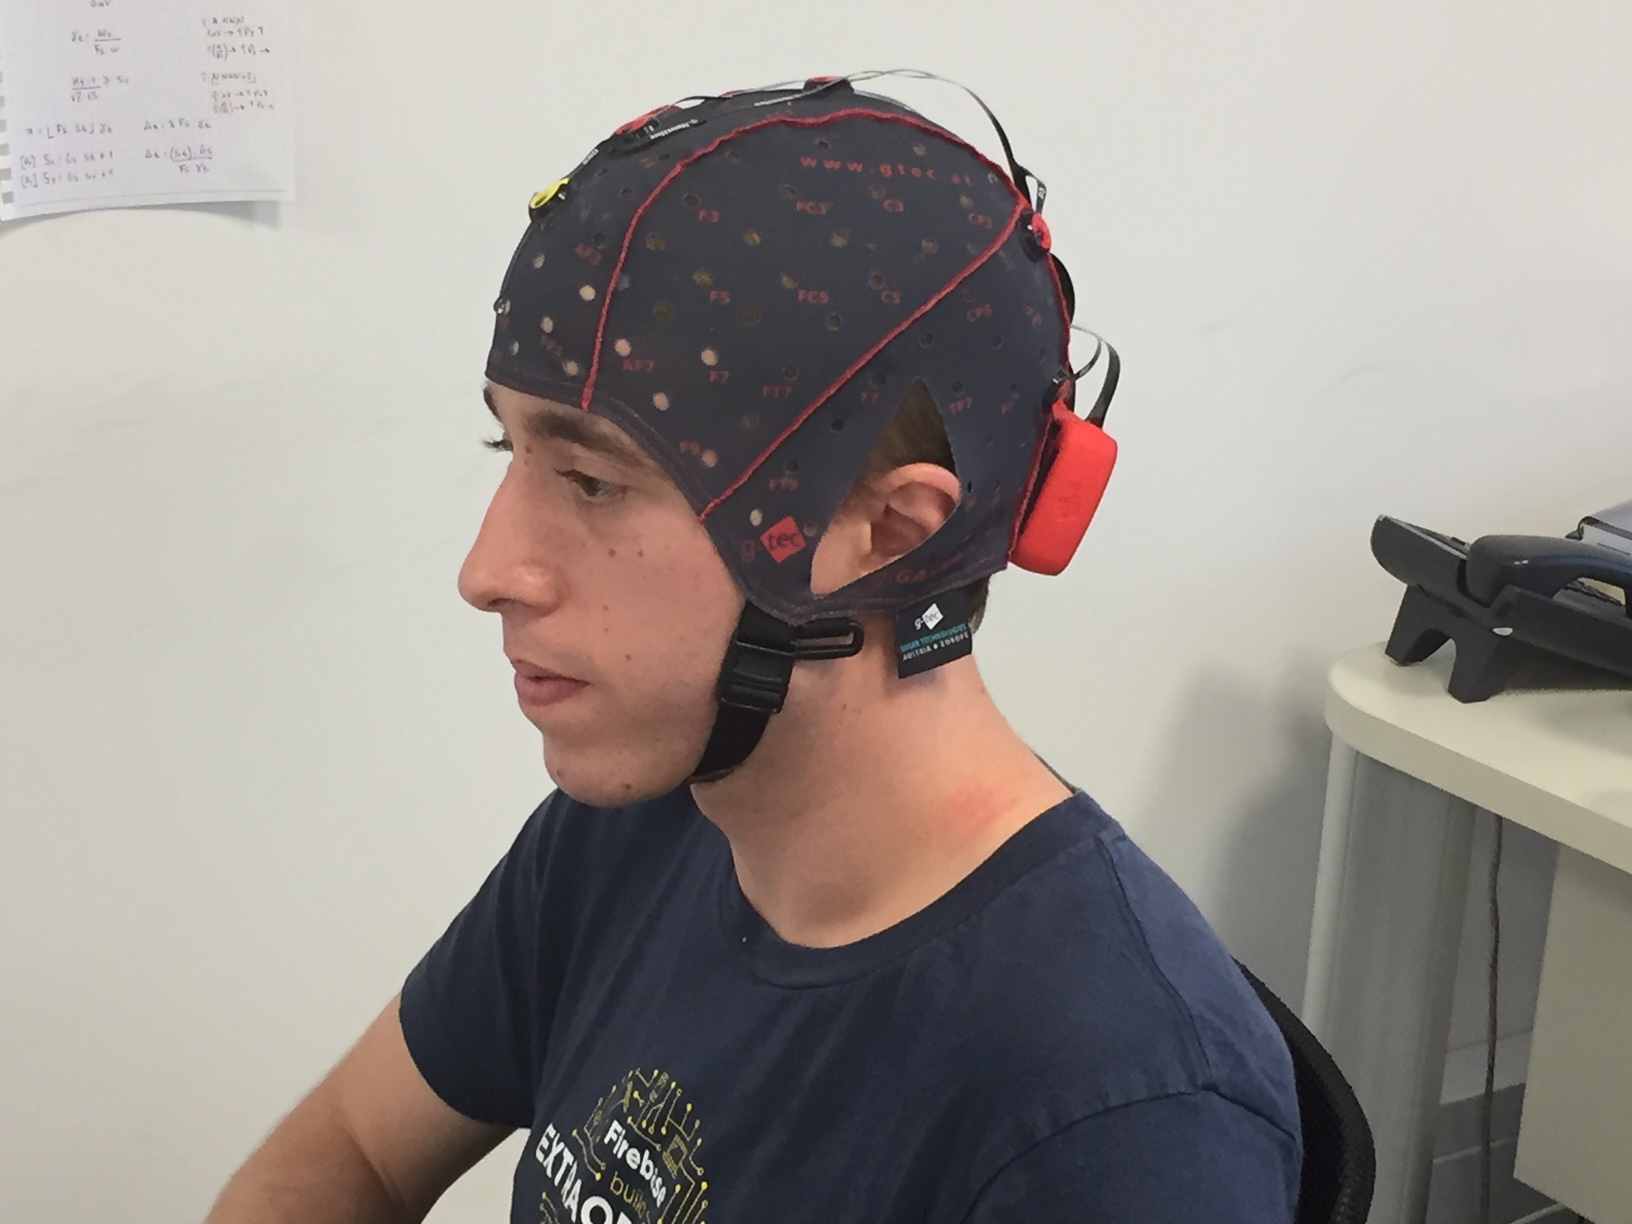
\includegraphics[width=0.8\linewidth]{gTecSubject.jpg}
\caption{Subject performing a P300 Speller experiment}
\end{figure}
\end{column}
\end{columns} % End of the subdivision

\begin{itemize}
\item Offline datasets
\begin{itemize}
\item Physiobank Alpha Wave
\item Motor Imagery BNCI-Horizon 002-2014
\item ALS P300 BNCI-Horizon 008-2014
\end{itemize}
\end{itemize}

\end{block}

%----------------------------------------------------------------------------------------
%	METHODS
%----------------------------------------------------------------------------------------

\begin{block}{Methods: Processing Pipeline and Feature Extraction}
\begin{enumerate}
\item Signal Preprocessing and Segmentation
\item Signal Plotting: single channel binary image 

\begin{align*}
I(z_1,z_2) = \left\{ \begin{array}{rl}
255 & \text{if} \,  z_1 = \gamma \cdot n; \; z_2 = EEG(n,c) + z(c) \\
0   & \mbox{otherwise}
\end{array}\right.
\label{eq:plotting}
\end{align*}

\begin{itemize}
\item \textbf{Bresenham} algorithm interpolates straight lines between consecutive sample points.
\end{itemize}

\begin{figure}[htb]
\centering
\subfigure[Patch over a Signal Complex]{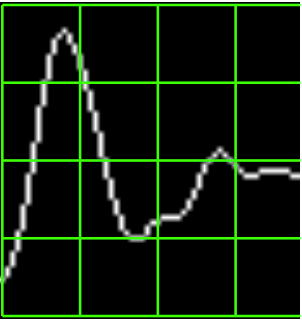
\includegraphics[width=.29\linewidth]{descriptorpatchsample}}
\subfigure[Gradient vector field around the signal]{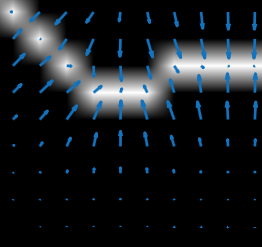
\includegraphics[height=316pt,width=.29\linewidth]{samplegradients}}
\subfigure[Oriented histogram on each block]{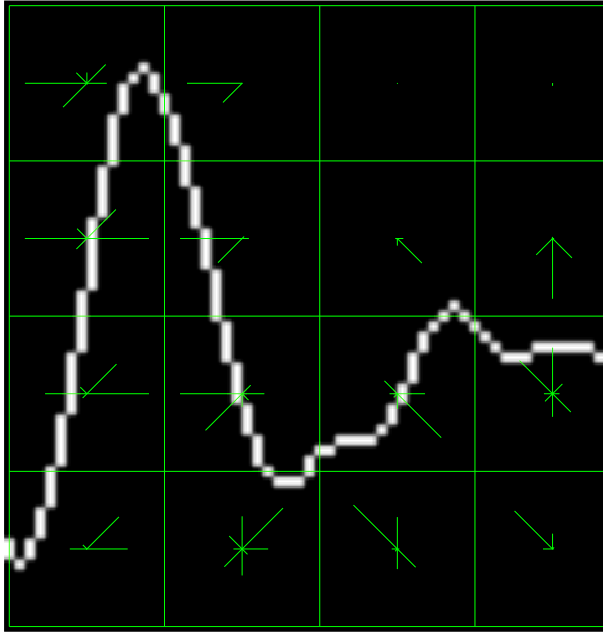
\includegraphics[width=.29\linewidth]{descriptorpatcharrows}}
\caption{Sample patch around a signal complex. The patch is divided in $4 \times 4$ blocks and $8$ orientations (bins) are calculated on each block, forming a $128$ normalized feature called \textit{descriptor}.}
\label{fig:histogramof}
\end{figure}


\item The Histogram of Gradient Orientations
\begin{itemize}
\item Popular and powerful tool from Computer Vision and basis of SIFT\textsuperscript{[5]} feature extraction method.
\item Inspired on how the visual cortex identify shapes.
\item For every pixel $\mathbf{p}$ on the image plot:
\end{itemize}

\begin{align*}
 h(\theta,i,j) = 3 s \sum_{\mathbf{p}} w_\mathrm{ang}(\angle J(\mathbf{p}) - \theta)\, w_{ij}\left(\frac{\mathbf{p} - \mathbf{kp}}{3 s}\right)\, |J(\mathbf{p})|
\end{align*}

\noindent with $s$ as the scale of the patch, $J(\mathbf{p})$ is the finite differences gradient vector, $ \theta \in \{0, 45, 90, 135, 180, 225, 270, 315\} $, $ i,j = \{0,1,2,3\} $, using the following trilinear interpolation functions \textsuperscript{[6]}

\begin{align*}
 w_{ij}(\mathbf{v}) = w( v_x - x_i ) w( v_y - y_i ) ,  w_\mathrm{ang}(\alpha) = \sum_{k} w( \frac{8\alpha}{2\pi} + 8r)
\end{align*}

\begin{align*}
 w(z) = \max(0,|z|-1)
\end{align*}


\end{enumerate}

\end{block}

%----------------------------------------------------------------------------------------
%	MATHEMATICAL SECTION
%----------------------------------------------------------------------------------------


%----------------------------------------------------------------------------------------

\end{column} % End of the first column

\begin{column}{.03\textwidth}\end{column} % Empty spacer column
 
\begin{column}{.465\textwidth} % The second column

%----------------------------------------------------------------------------------------
%	RESULTS
%----------------------------------------------------------------------------------------

\begin{block}{Methods: Classification}

\begin{itemize}
\item Straightforward supervised classification model based on \textbf{Naive Bayes Near Neighbor}.
\begin{itemize}
\item Binary (oscillatory) or unary (transient) classification
\end{itemize}
\item For \textit{descriptors} $ d_i $ obtained from test signals, the class where the image (and the signal) belongs can be inferred by resolving

\begin{align*}
\hat{C} = \arg \min_C \big\{\sum_{}^{} \left\lVert d_i - NN_C(d_i) \right\rVert ^2 \big\}
\end{align*}

\item where $NN_C(d_i)$ are the set of prototype descriptors.
\end{itemize}

\end{block}

\begin{block}{Results}

\begin{itemize}
\item Transient and oscillatory phenomena have been studied.
\end{itemize}

\begin{table}
\begin{tabular}{l l l}
\toprule
\textbf{Waveform} & \textbf{Best ACC} & \textbf{Intra-Subject Avg}\\
\midrule
$\mu$ & $75\%$ & $65\%$ \\
P300  & $95\%$ & $45\%$ \\
$\alpha$  & $95\%$ & $80\%$ \\
\bottomrule
\end{tabular}
\caption{Classification Accuracy percentage}
\end{table}

%\begin{itemize}
%\item Sollicitudin Vel Orci
%\item Maecenas Ultricies Feugiat Velit Non Mattis.
%\end{itemize}
     
\end{block}

%------------------------------------------------

\begin{block}{Results}

\begin{figure}[htb]
\centering
\subfigure[$\alpha$ Wave]{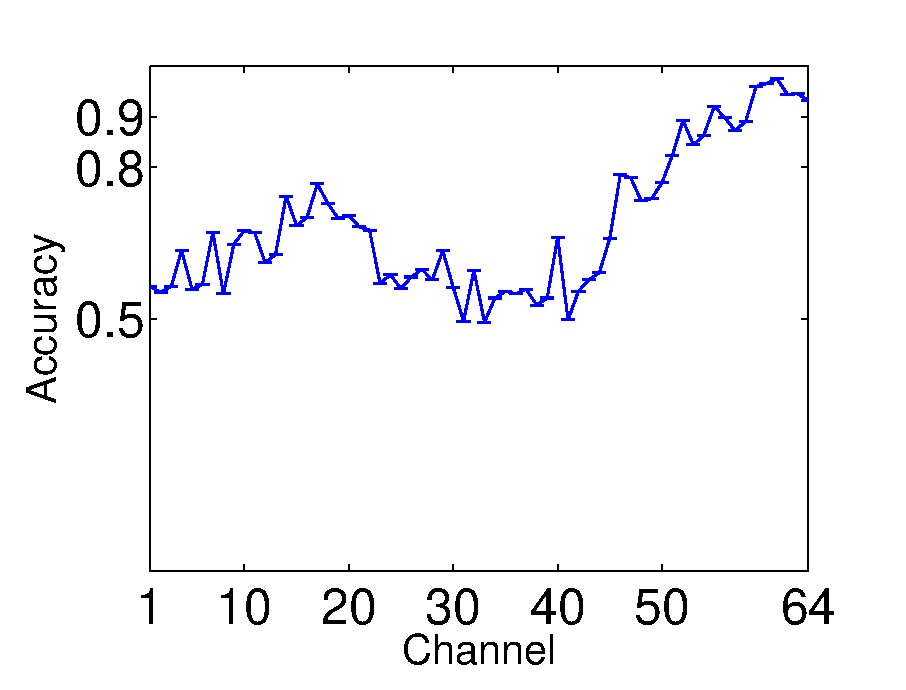
\includegraphics[width=.32\linewidth]{DatasetPhysionetAccuracyPerChannel.eps}}
\subfigure[$\mu$ Wave]{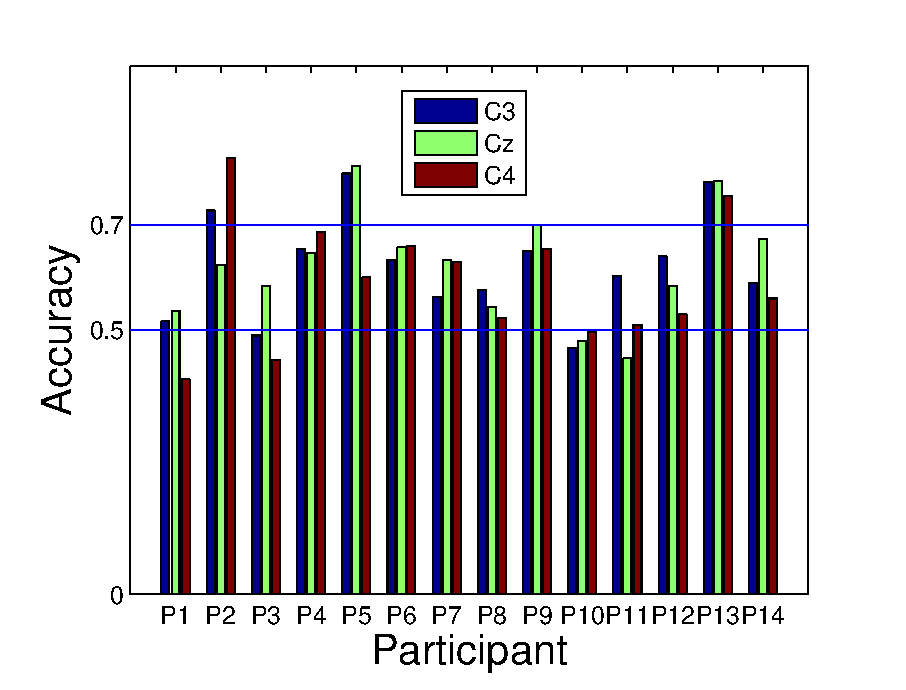
\includegraphics[width=.32\linewidth]{DatasetMICrossValidation2.eps}}
\subfigure[P300]{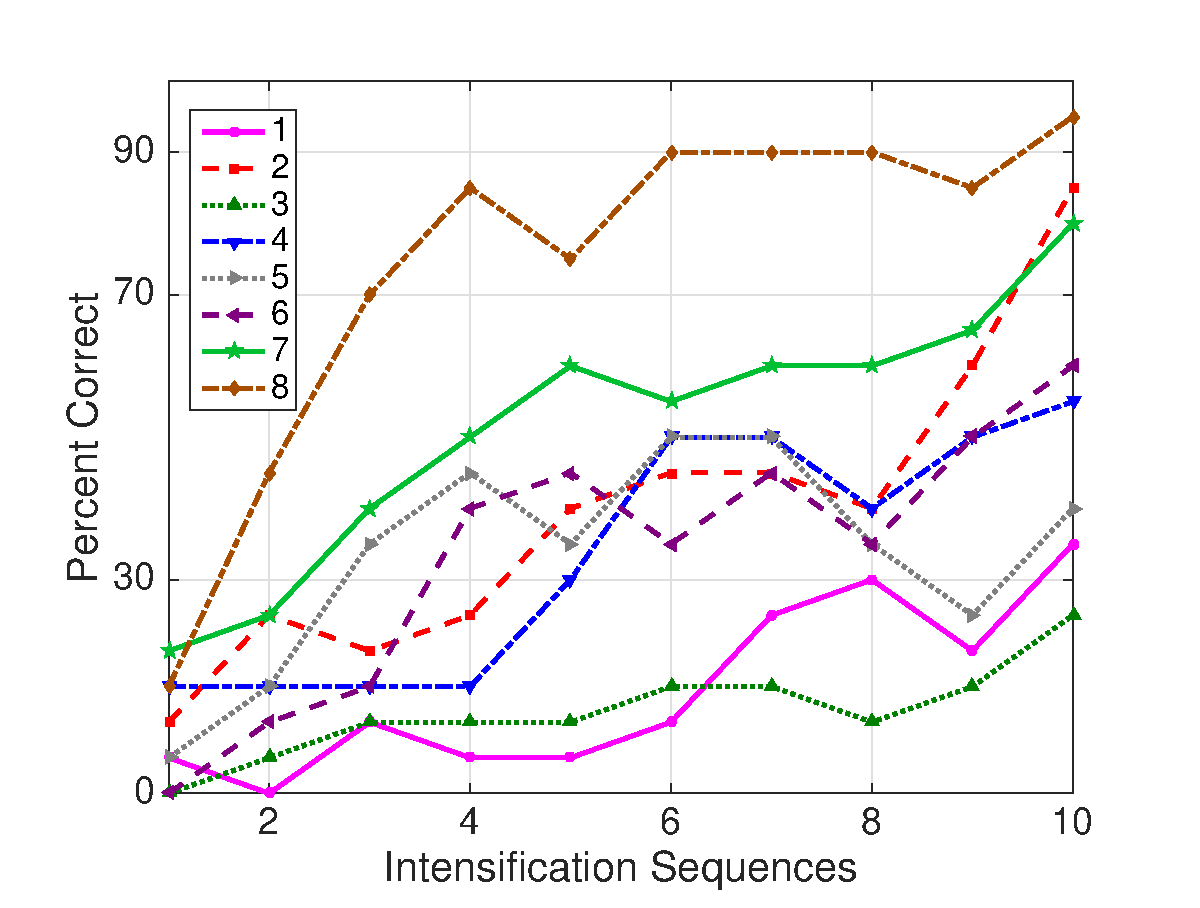
\includegraphics[width=.32\linewidth]{performance2.eps}}
\caption{Classification accuracy percentages.}
\label{fig:p300matrix}
\end{figure}
\end{block}

%----------------------------------------------------------------------------------------
%	CONCLUSION
%----------------------------------------------------------------------------------------

\begin{block}{Significance}

\begin{itemize}
\item A method which is biomimetically based on how the visual cortex works by detecting orientations, ironically, is used preciely to detect information from the brain.
\item It has universal applicability because the same basic methodology can be applied to detect different patterns in EEG for BCI
\item It has the potential to foster close collaboration with physicians and electroencephalograph technicians.
\item Follows the established procedure of the clinical EEG of analyzing waveforms by their shapes.
\item Eases the clinical acceptance and use of qEEG technologies.
\end{itemize}

\end{block}

%----------------------------------------------------------------------------------------
%	REFERENCES
%----------------------------------------------------------------------------------------

\begin{block}{References}
              \begin{itemize}
                \item [1] \small Guger C., Allison B.Z., Lebedev M.A. (2017) Recent Advances in Brain-Computer Interface Research A Summary of the BCI Award 2016 and BCI Research Trends.
                \item [2] Alvarado-González, M.; Garduño, E.; Bribiesca, E.; Yáñez-Suárez, O.; MedinaBañuelos, V. P300 Detection Based on EEG Shape Features. 2016
                \item [3] Zhang J.; Zou J.; Automatic detection of interictal epileptiform discharges based on time-series sequence merging method, Neurocomputing, 2013;
                \item [4] Ramele, R.; Villar, A.J.; Santos, J.M. BCI classification based on signal plots and SIFT descriptors. 2016;
                \item [5] D. G. Lowe, Object recognition from local scale-invariant features.1999
                \item [6] Vedaldi, A.; Fulkerson, B. VLFeat - An open and portable library of computer vision algorithms. Design 2010;
                \item [7] Chavarriaga et al; Heading for new shores! Overcoming pitfalls in BCI design, Brain-Computer Interfaces, TF 2016;
              \end{itemize}
                      
%\nocite{*} % Insert publications even if they are not cited in the poster
%\small{\bibliographystyle{unsrt}
%\bibliography{sample}}

\end{block}

%----------------------------------------------------------------------------------------
%	ACKNOWLEDGEMENTS
%----------------------------------------------------------------------------------------

\begin{block}{Acknowledgments}

\begin{itemize}
\item This project was supported by the ITBACyT-15 funding program issued by ITBA University in Buenos Aires, Argentina
\end{itemize}

\end{block}

%----------------------------------------------------------------------------------------
%	CONTACT INFORMATION
%----------------------------------------------------------------------------------------


%\begin{block}{Contact Information}
%
%\begin{itemize}
%\item Web: \href{https://www.itba.edu.ar/id/centro-de-inteligencia-computacional/}{CiC@ITBA}
%\item Email: \href{mailto:rramele@itba.edu.ar}{rramele@itba.edu.ar}
%\item Phone: +54 (911) 4193 9382
%\end{itemize}
%
%\end{block}

%----------------------------------------------------------------------------------------

\end{column} % End of the second column

\begin{column}{.015\textwidth}\end{column} % Empty spacer column

\end{columns} % End of all the columns in the poster

\end{frame} % End of the enclosing frame

\end{document}